\documentclass[]{article}
\usepackage{amsmath}
\usepackage{listings}
\usepackage{float}
\usepackage{graphicx}

\begin{titlepage}
\author{Darryen Sands}
\title{Matched Filtering Analysis and Wave Generation Summary}
\end{titlepage}

\begin{document}
This will be a short summary of how to perform matchfiltering analysis and how to generate wave signals. \\

Let's perform match filtering analysis on GW151226. This wave was detected on December 25 2015, at 3:38:53 UTC. To do this we implement the following code:

\begin{lstlisting}[language = Python]
from pycbc.frame import read_frame
from pycbc.filter import highpass_fir, lowpass_fir, matched_filter
from pycbc.waveform import get_fd_waveform
from pycbc.psd import welch, interpolate
from pycbc.catalog import Merger
import pylab 

#Whitening Strain
for ifo in ['H1', 'L1']:
    h1 = Merger("GW151226").strain(ifo)
    h1 = highpass_fir(h1, 15, 8)

    psd = interpolate(welch(h1), 1.0/ h1.duration)

    white_strain = (h1.to_frequencyseries() / psd ** 0.5).to_timeseries()
    
    smooth = highpass_fir(white_strain, 35, 8)
    smooth = lowpass_fir(white_strain, 300, 8)

    if ifo == 'L1':
        smooth *= -1 
        smooth.roll(int(.007 / smooth.delta_t))


    pylab.plot(smooth.sample_times, smooth, label = ifo)
pylab.legend()
pylab.xlim(1135136350.60,1135136350.67)
pylab.ylim(-150, 150)
pylab.ylabel('Smoothed-Whitened Strain')
pylab.grid()
pylab.xlabel('GPS Time (s)')
pylab.show()
\end{lstlisting}

This code displays how to whiten the strain. What does whitening the strain mean? Whitening the data removes noise from both the high and low frequencies. We'll have an area from around 80-300 Hz that is mostly flat (i.e. the whitened area). Ultimately, since gravitational waves are so weak we need to remove as much noise as possible to detect them. \\

The above code imports the strain data from both the Livingston and Hanford detectors. We apply a high pass filter to remove low frequency noise and we calculate the power spectral density using Welch's function. Welch's function acts a sliding window to view our power spectral density (PSD) at different frequencies to get an accurate estimate. We finally smooth out the data and plot it. The plot is below. \\

\begin{figure}[H]
	\begin{center}
		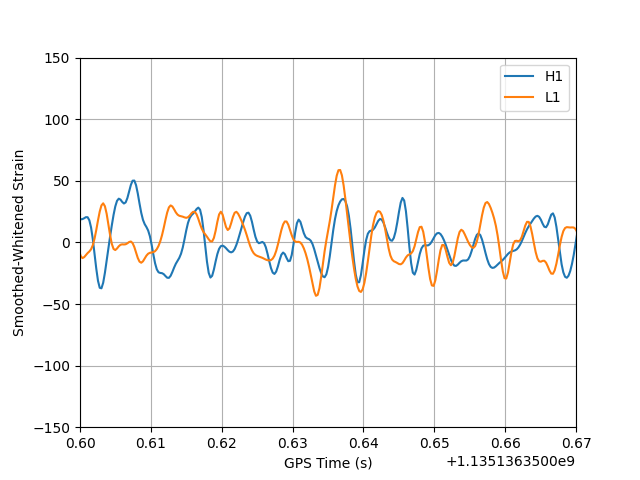
\includegraphics[scale=1]{WhitenStrain.png}
	\end{center}
	\caption{The whitened strain data.}
	\label{fig:whitedata}
\end{figure}

The next thing we need to do is calculate a signal-to-noise ratio (SNR) and we can do that with the following code:

\begin{lstlisting}[language = Python]
hp, hc = get_fd_waveform(approximant = "IMRPhenomD", mass1 = 14.2, mass2 = 7.5, f_lower = 20, delta_f = 1.0/h1.duration)

hp.resize(len(h1) // 2 + 1)

snr = matched_filter(hp,h1,psd=psd, low_frequency_cutoff = 20.0)
snr = snr[len(snr) // 4: len(snr) * 3 // 4]

pylab.plot(snr.sample_times, abs(snr))
pylab.ylabel('Signal-to-Noise')
pylab.xlabel('GPS Time (s)')
pylab.savefig("SNR.png")
pylab.show()
\end{lstlisting}

The above code works by defining a template wave that our signal could be represented by. After this step we calculate the SNR and plot the results.

\begin{figure}[H]
	\begin{center}
		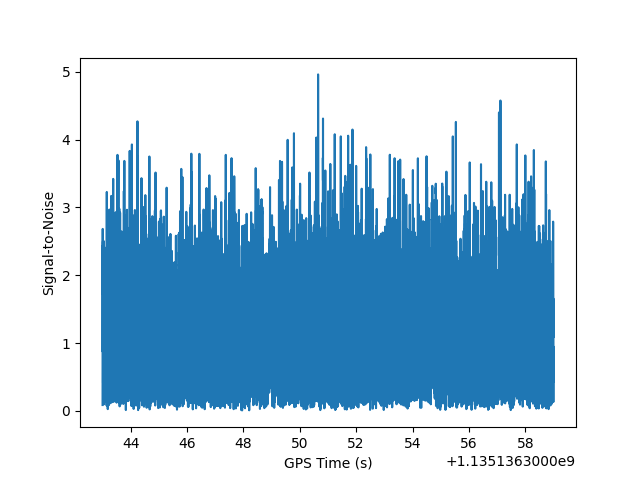
\includegraphics[scale=1]{SNR.png}
	\end{center}
	\caption{The signal-to-noise ratio. The signal is quite weak and this could mean that the noise overpowers the signal.}
	\label{fig:SNR}
\end{figure}

This signal that we received is not the greatest as it doesn't capture the signal at all. \\

Now we will move on to generating wave signals. We actually did this when we tried to perform matched filtering. The get\_fd\_waveform and get\_td\_waveform allows us to create a template wave using different approximation methods. We must provide the function the masses of the black holes, the spins of the black holes, the area where the black holes are located (right ascension, inclination), the starting frequency, and the time between samples. Other parameters can be given but these are the main ones.
 
The code for generating a wave signal is like the following:

\begin{lstlisting}[language = Python]
hp, hc = get_td_waveform(approximant="SEOBNRv4_opt",
                         mass1=10,
                         mass2=100,
                         delta_t=1.0/4096,
                         f_lower=20)

pylab.plot(hp.sample_times, hp, label='Plus Polarization')
pylab.plot(hp.sample_times, hc, label='Cross Polarization')
pylab.xlabel('Time (s)')
pylab.legend()
pylab.grid()
pylab.show()

# Zoom in near the merger time#
pylab.plot(hp.sample_times, hp, label='Plus Polarization')
pylab.plot(hp.sample_times, hc, label='Cross Polarization')
pylab.xlabel('Time (s)')
pylab.xlim(-.01, .01)
pylab.legend()
pylab.grid()
pylab.show()
\end{lstlisting}

\begin{figure}[H]
	\begin{center}
		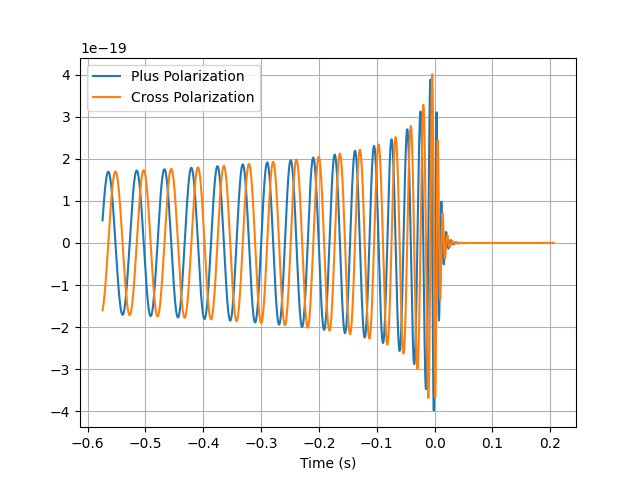
\includegraphics[scale=1]{HPHC.png}
	\end{center}
	\caption{Both of the cross and plus polarizations. This is what the sample waveform looks like with the given parameters.}
	\label{fig:HPHC}
\end{figure}

\begin{figure}[H]
	\begin{center}
		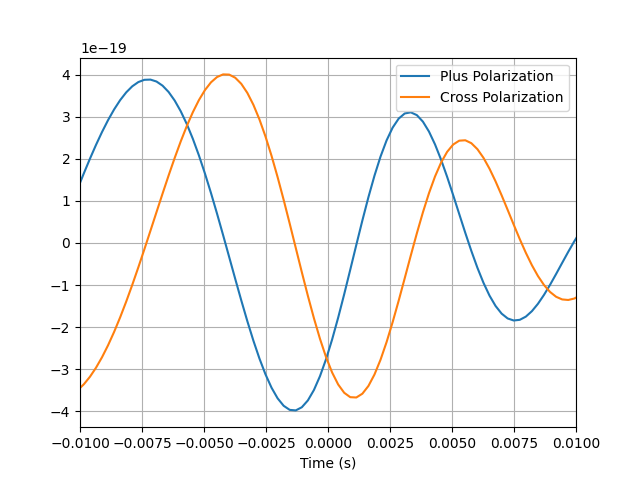
\includegraphics[scale=1]{HPHCClose.png}
	\end{center}
	\caption{A closer view of those same cross and plus polarizations with the given parameters.}
	\label{fig:HPHCClose}
\end{figure}


\end{document}